\section{Results}
\label{sec:results}
\subsection{Downsampling}
With data from G2M2, k-NN prediction running times
were measured vs. dataset size N at various DPI.
The results
are presented in figure \ref{fig:knn-runningtime-vs-n-and-k}.
\begin{figure}[ht]
	\centering
	\begin{subfigure}{0.5\textwidth}
		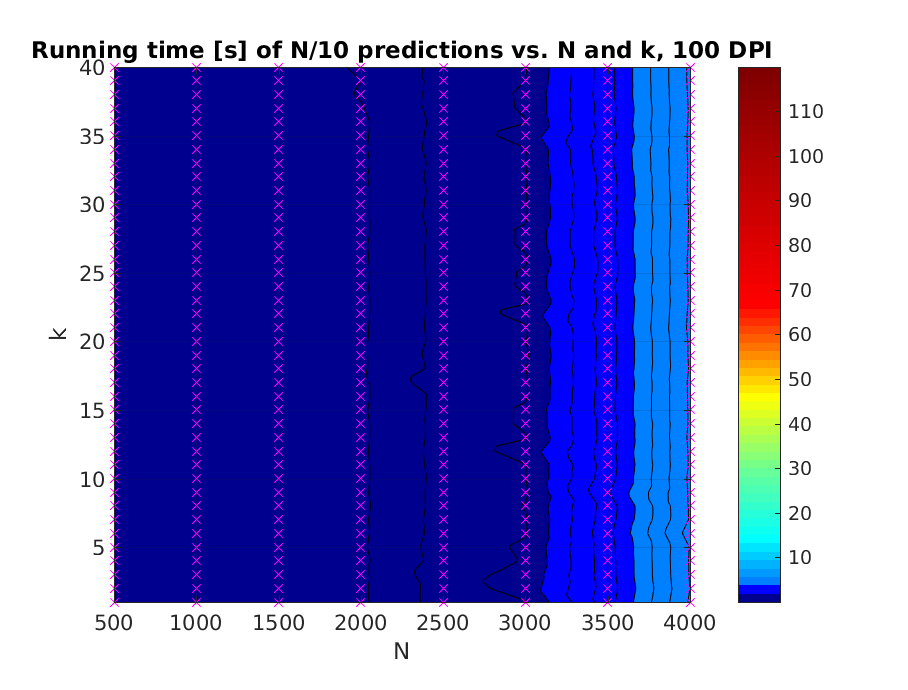
\includegraphics[width = \textwidth]{img/knn-runningTimeVsKVSN-G2M2-dpi100}
		\caption{100 DPI}
	\end{subfigure}
	\begin{subfigure}{0.5\textwidth}
		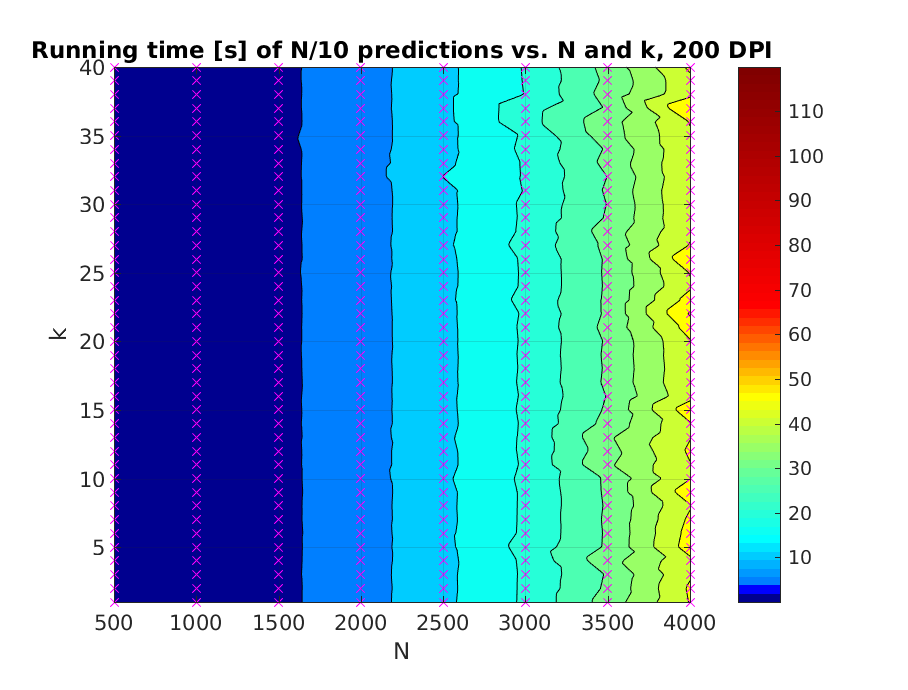
\includegraphics[width = \textwidth]{img/knn-runningTimeVsKVSN-G2M2-dpi200}
		\caption{200 DPI}
	\end{subfigure}
	\begin{subfigure}{0.5\textwidth}
		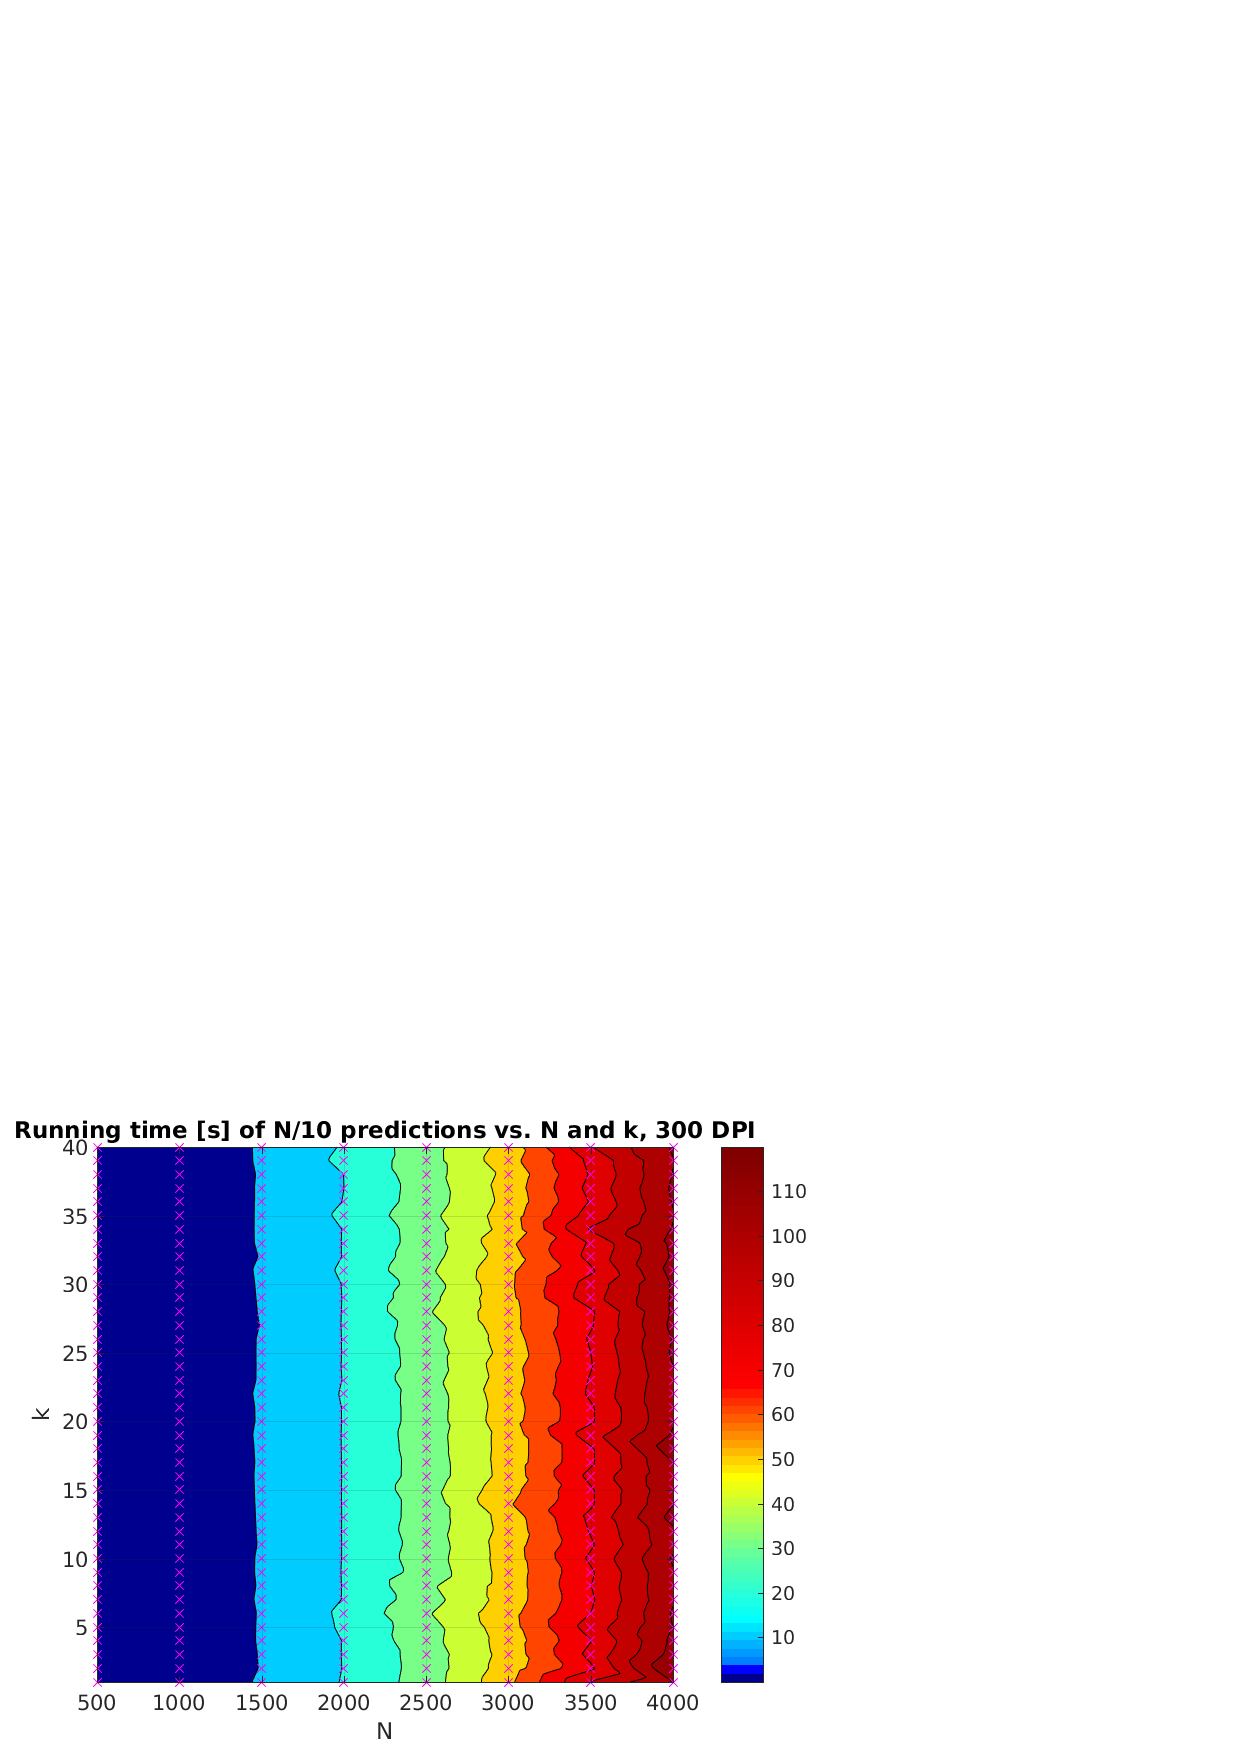
\includegraphics[width = \textwidth]{img/knn-runningTimeVsKVSN-G2M2-dpi300}
		\caption{300 DPI}
	\end{subfigure}
	\caption[
	k-NN prediction running time
			vs. dataset size N and k at various DPI.
	]{
		k-NN prediction running time in seconds
		vs. dataset size N and k for G2M2 data at various DPI.
		}
	\label{fig:knn-runningtime-vs-n-and-k}
\end{figure}

It is clearly seen that running times are much reduced by downsampling,
and that running times increase substantially with N. It is also seen that
the running times do not vary with k.
Figure \ref{fig:knn-runningtime-vs-n-loglog} visualizes the relationship
between running time and N further.
\begin{figure}[ht]
	\centering
	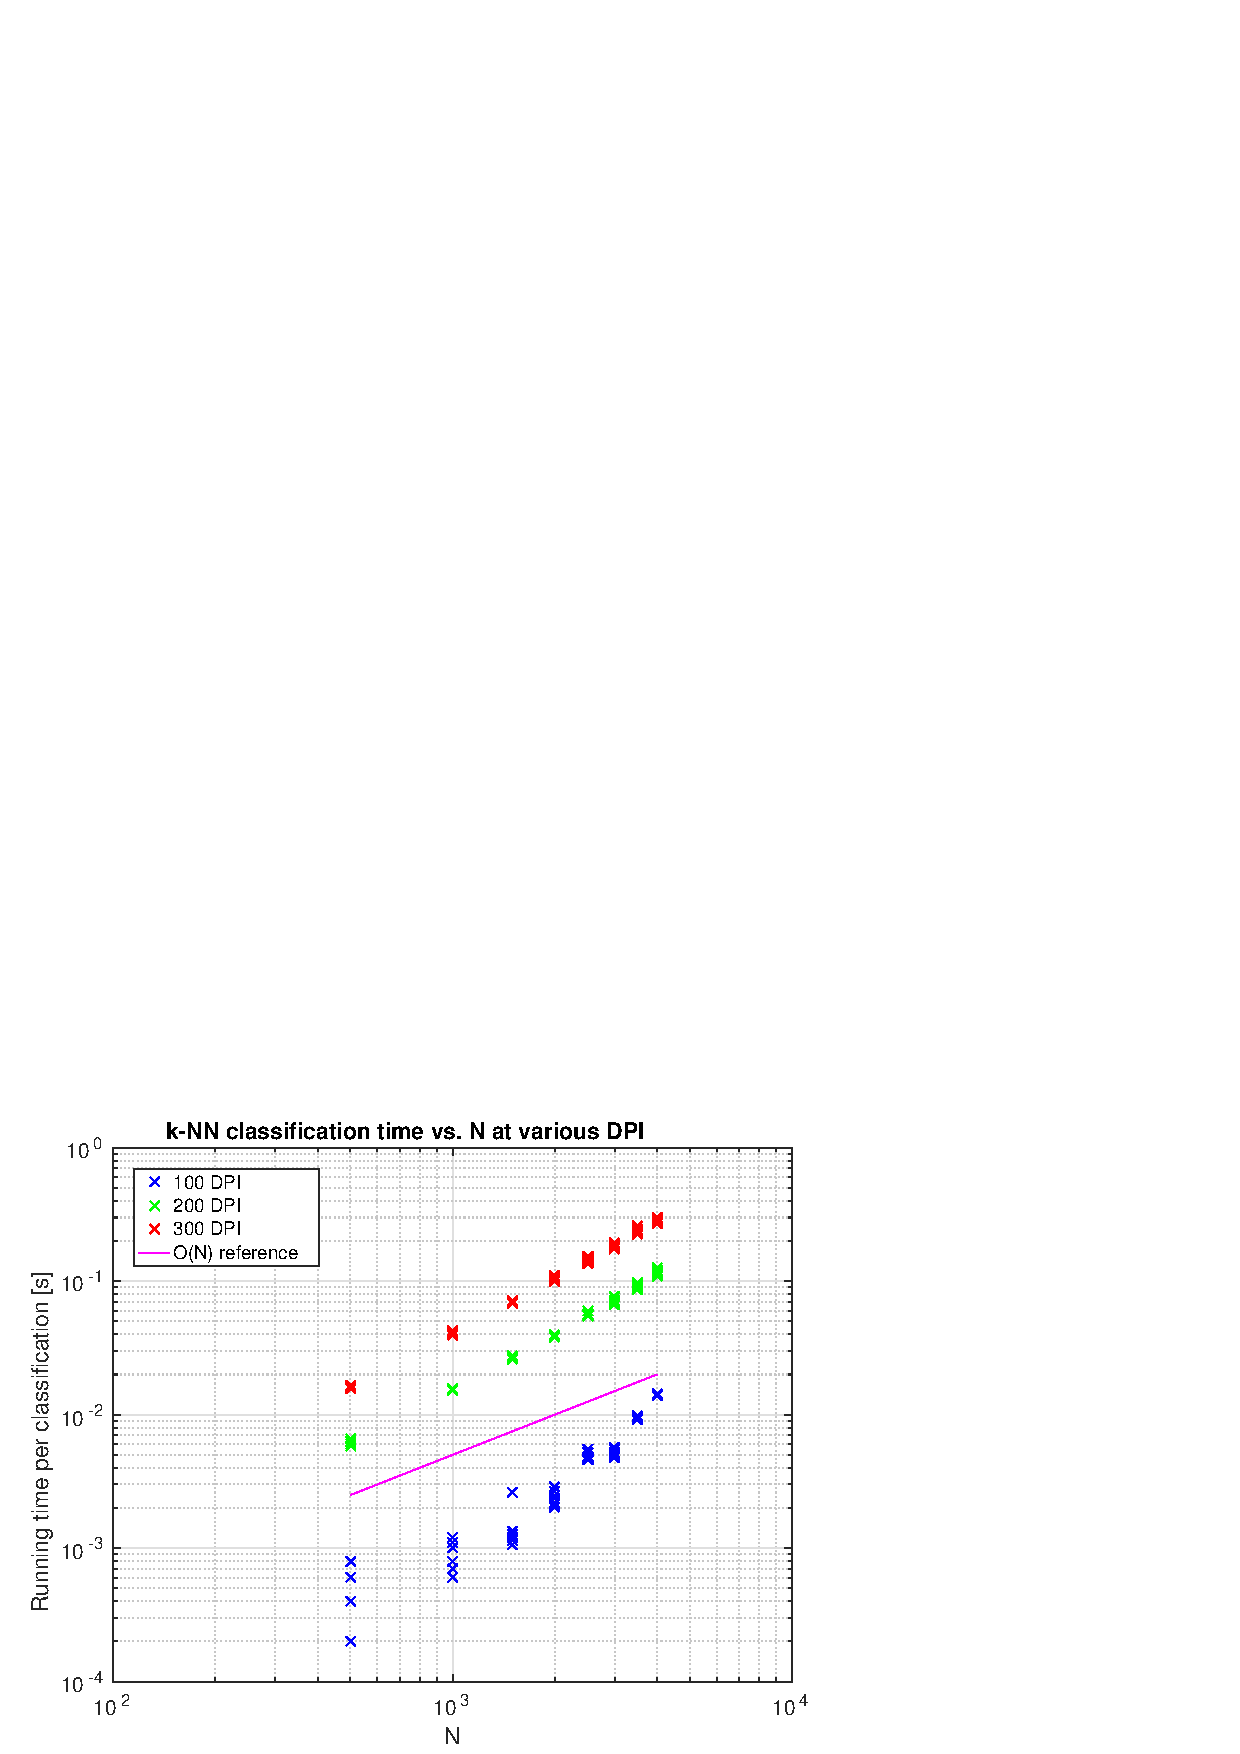
\includegraphics[width = 0.5\textwidth]{img/knn-runningTimeVsNVsDPI-G2M2}
	\caption[log-log plot of k-NN prediction running time vs. N at various DPI.]{
		log-log plot of k-NN prediction running time in seconds vs. N at various DPI.
		\(5\cdot{}10^{-6}\cdot{}N\) reference line also plotted.
	}
	\label{fig:knn-runningtime-vs-n-loglog}
\end{figure}

It can be seen from figure \ref{fig:knn-runningtime-vs-n-loglog} that
the classification time complexity is larger than \(O(N)\).

\subsection{Smoothing}
Figure \ref{fig:knn-AccVsKVsSigma-G2M2},
displays k-NN prediction accuracy vs. smoothing parameter \(\sigma\)
and number of neighbours k on the G2M2 dataset, at various pixel densities.
It is observed that classification accuracies above 0.995
are obtained at all three pixel densities, with different \(\sigma\).
\begin{figure}[ht]
	\centering
	\begin{subfigure}{0.46\textwidth}
		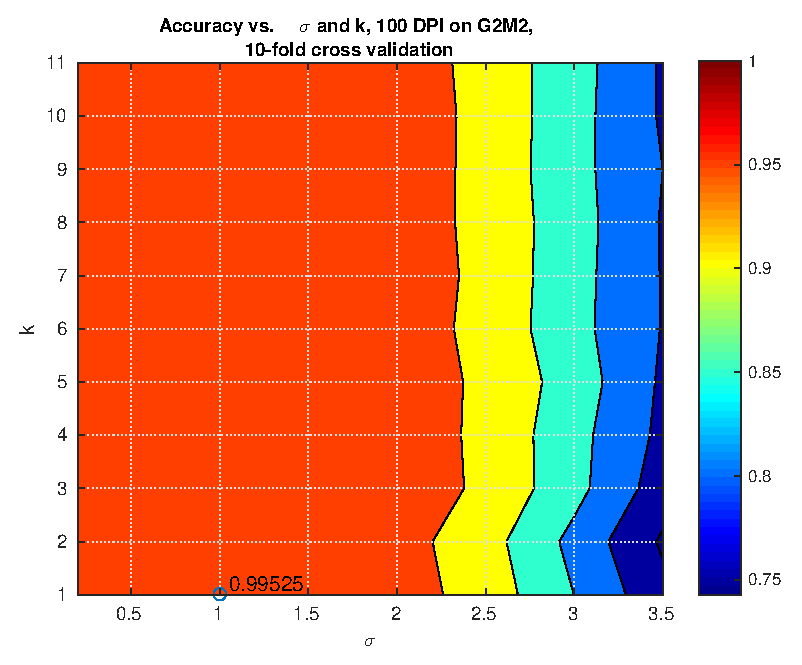
\includegraphics[width = \textwidth]{img/knn-AccVsKVsSigma-G2M2-dpi100-cv10}
		\caption{100 DPI}
	\end{subfigure}
	\begin{subfigure}{0.46\textwidth}
		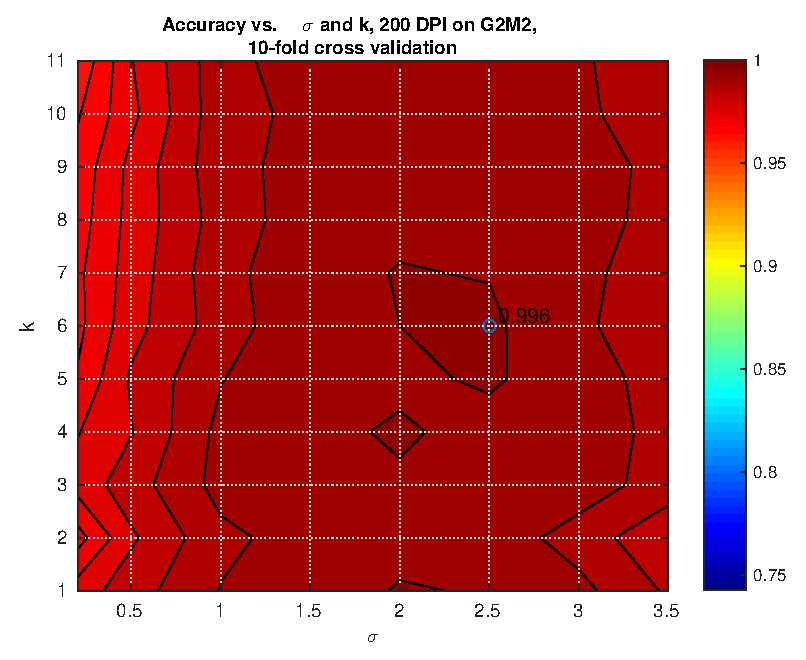
\includegraphics[width = \textwidth]{img/knn-AccVsKVsSigma-G2M2-dpi200-cv10}
		\caption{200 DPI}
	\end{subfigure}
	\begin{subfigure}{0.46\textwidth}
		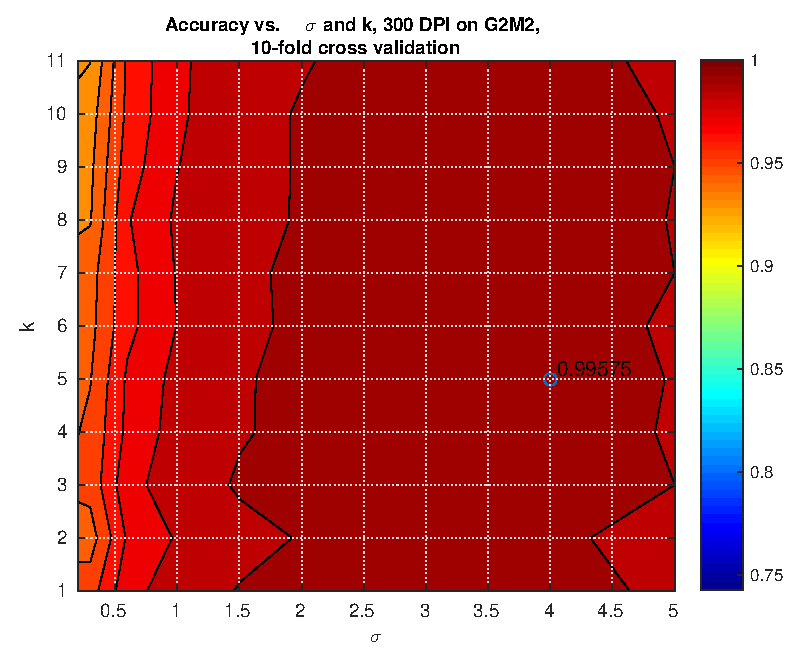
\includegraphics[width = \textwidth]{img/knn-AccVsKVsSigma-G2M2-dpi300-cv10}
		\caption{300 DPI}
	\end{subfigure}
	\caption[k-NN prediction accuracy vs. smoothing parameter $\sigma$
			and k at various DPI.]{
		k-NN prediction accuracy vs. smoothing parameter $\sigma$
		and k for G2M2 data at various DPI.
		}
	\label{fig:knn-AccVsKVsSigma-G2M2}
\end{figure}

\clearpage
\subsection{Principal Component Analysis}
Figure \ref{fig:principal-components} shows the first ten principal
components for all the data, at various DPI.
The normalized intensity \(I_i\) of each pixel in the PC visualization
depends on the weighed contribution \(w_i\) of the pixel position to the principal component
and is determined by
\(I_i=\frac{\left|w_i\right|-\left|w\right|_{min}}{\left|w\right|_{max}-\left|w\right|_{min}}\)
.
\begin{figure}[ht]
\centering
\setlength\tabcolsep{1pt}
\begin{tabular}{r*{10}{c}}
Preprocessing & PC1 & PC2 & PC3 & PC4 & PC5 & PC6 & PC7 & PC8 & PC9 & PC10 \\
100 DPI, \(\sigma\)=1
 & 
\includegraphics[width=\smallfigscale]{img/pca-All-dpi100-sigma1-pc1} 
 & 
\includegraphics[width=\smallfigscale]{img/pca-All-dpi100-sigma1-pc2} 
 & 
\includegraphics[width=\smallfigscale]{img/pca-All-dpi100-sigma1-pc3} 
 & 
\includegraphics[width=\smallfigscale]{img/pca-All-dpi100-sigma1-pc4} 
 & 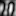
\includegraphics[width=\smallfigscale]{img/pca-All-dpi100-sigma1-pc5} 
 & 
\includegraphics[width=\smallfigscale]{img/pca-All-dpi100-sigma1-pc6} 
 & 
\includegraphics[width=\smallfigscale]{img/pca-All-dpi100-sigma1-pc7} 
 & 
\includegraphics[width=\smallfigscale]{img/pca-All-dpi100-sigma1-pc8} 
 & 
\includegraphics[width=\smallfigscale]{img/pca-All-dpi100-sigma1-pc9} 
 & 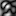
\includegraphics[width=\smallfigscale]{img/pca-All-dpi100-sigma1-pc10} 
\\
200 DPI, \(\sigma\)=2.5
 & 
\includegraphics[width=\smallfigscale]{{img/pca-All-dpi200-sigma2.5-pc1}.png} 
 & 
\includegraphics[width=\smallfigscale]{{img/pca-All-dpi200-sigma2.5-pc2}.png} 
 & 
\includegraphics[width=\smallfigscale]{{img/pca-All-dpi200-sigma2.5-pc3}.png} 
 & 
\includegraphics[width=\smallfigscale]{{img/pca-All-dpi200-sigma2.5-pc4}.png} 
 & 
\includegraphics[width=\smallfigscale]{{img/pca-All-dpi200-sigma2.5-pc5}.png} 
 & 
\includegraphics[width=\smallfigscale]{{img/pca-All-dpi200-sigma2.5-pc6}.png} 
 & 
\includegraphics[width=\smallfigscale]{{img/pca-All-dpi200-sigma2.5-pc7}.png} 
 & 
\includegraphics[width=\smallfigscale]{{img/pca-All-dpi200-sigma2.5-pc8}.png} 
 & 
\includegraphics[width=\smallfigscale]{{img/pca-All-dpi200-sigma2.5-pc9}.png} 
 & 
\includegraphics[width=\smallfigscale]{{img/pca-All-dpi200-sigma2.5-pc10}.png} 
\\
300 DPI, \(\sigma\)=4
 & 
\includegraphics[width=\smallfigscale]{img/pca-All-dpi300-sigma4-pc1} 
 & 
\includegraphics[width=\smallfigscale]{img/pca-All-dpi300-sigma4-pc2} 
 & 
\includegraphics[width=\smallfigscale]{img/pca-All-dpi300-sigma4-pc3} 
 & 
\includegraphics[width=\smallfigscale]{img/pca-All-dpi300-sigma4-pc4} 
 & 
\includegraphics[width=\smallfigscale]{img/pca-All-dpi300-sigma4-pc5} 
 & 
\includegraphics[width=\smallfigscale]{img/pca-All-dpi300-sigma4-pc6} 
 & 
\includegraphics[width=\smallfigscale]{img/pca-All-dpi300-sigma4-pc7} 
 & 
\includegraphics[width=\smallfigscale]{img/pca-All-dpi300-sigma4-pc8} 
 & 
\includegraphics[width=\smallfigscale]{img/pca-All-dpi300-sigma4-pc9} 
 & 
\includegraphics[width=\smallfigscale]{img/pca-All-dpi300-sigma4-pc10} 
\end{tabular}
\caption[Principal components at various DPI.]
{Principal components at various DPI.}
\label{fig:principal-components}
\end{figure}

It is observed that the principal components are very similar
at the three pixel densities, up until principal component 7,
at which point differences are more clearly seen.
It is also observed that the principal components
weigh pixels from all parts of the images, not just the borders.

Figure \ref{fig:pca-cumvar} shows the cumulated proportion of variance
explained vs. the number of principal components used for data representation,
based on an analysis of all data.
The elbow point is observed at a cumulated variance of approximately 0.95.
\begin{figure}[ht]
\centering
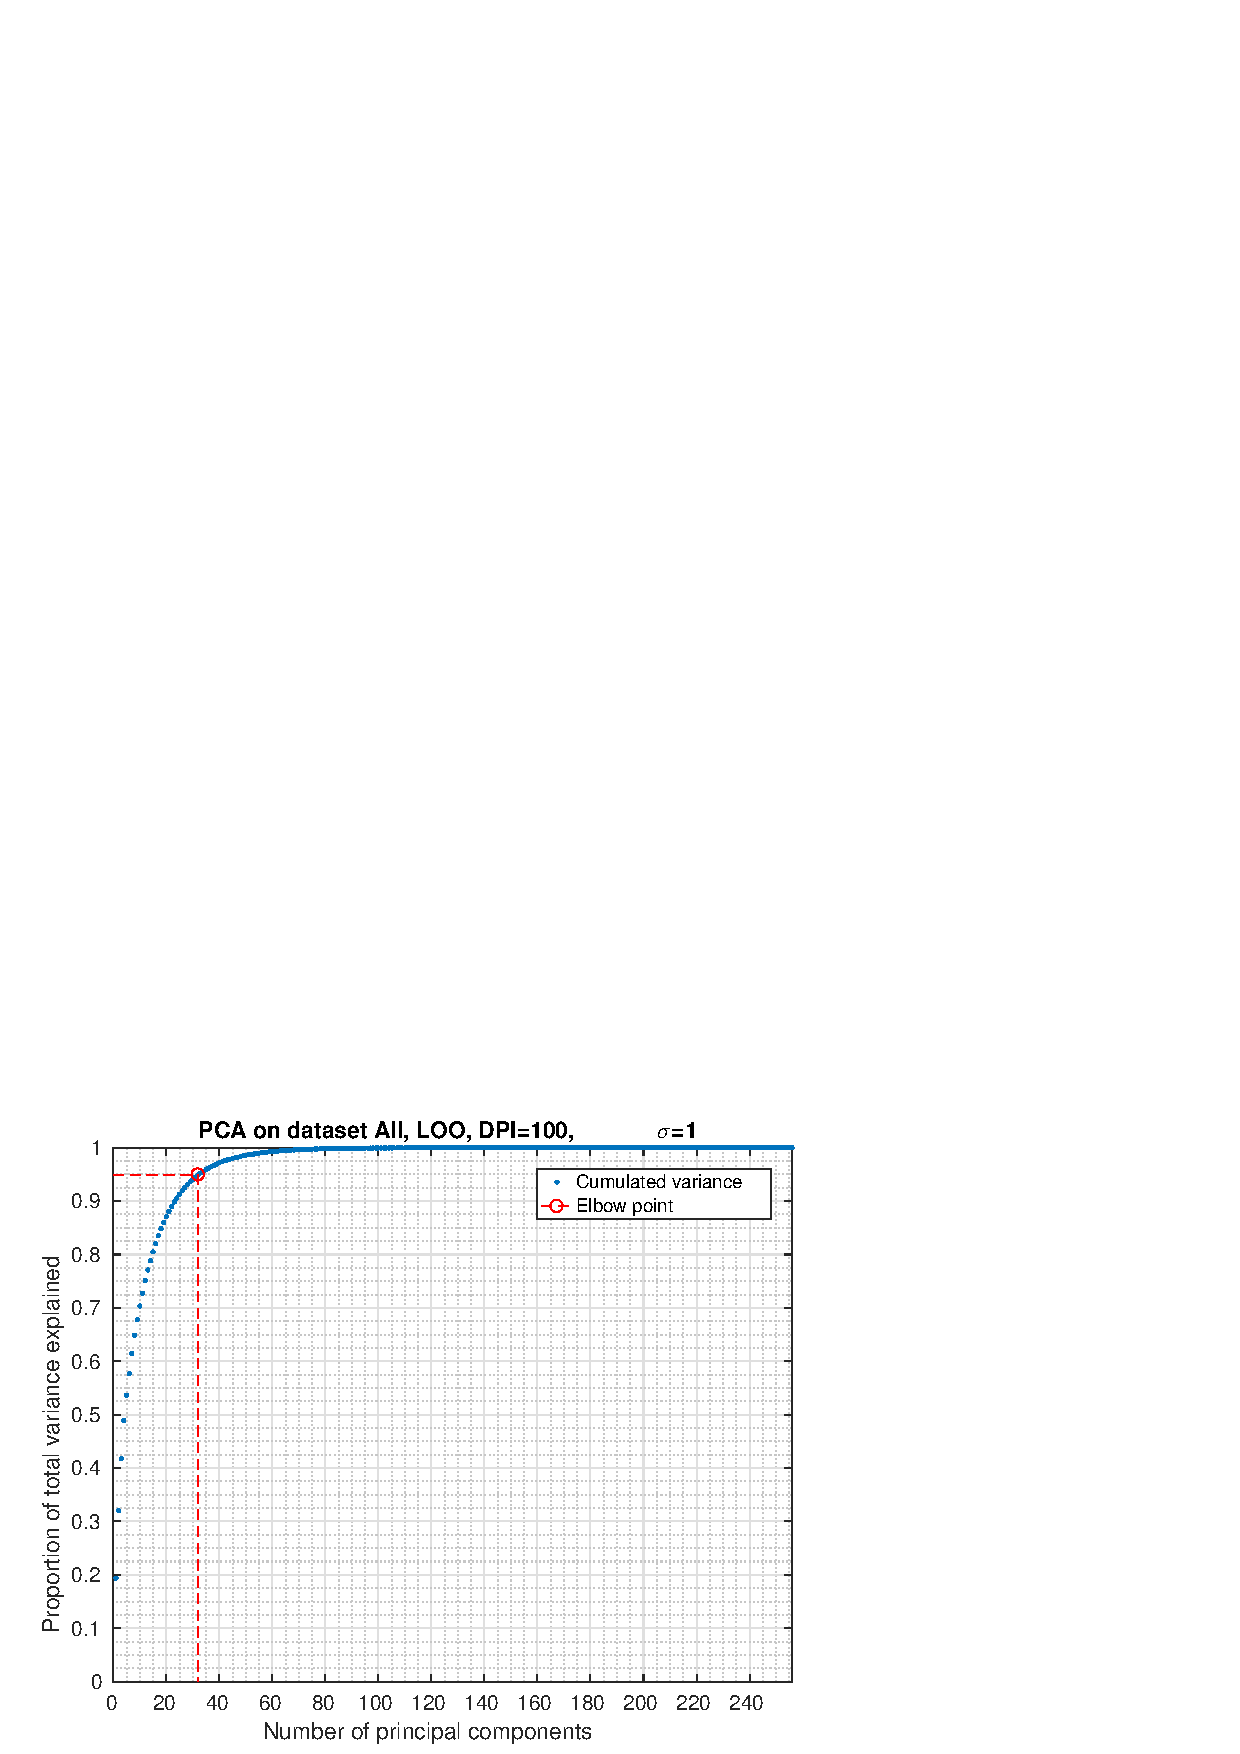
\includegraphics[width=\figscale]{img/pca-All-cumvar-dpi100-sigma1}
\caption[Cumulated variance explained by PCA]
{Cumulated proportion of variance explained vs. number of principal components.
All data was used for the analysis, preprocessed with DPI=100 and \(\sigma=1\).}
\label{fig:pca-cumvar}
\end{figure}

\subsection{Parameter optimization}
Figure \ref{fig:pca-knn-acc-vs-k} shows k-NN classification
accuracy vs. number of neighbours k on the \(D_{FEWER}\) dataset.
It is observed that the accuracy is maximal with k=5.
\begin{figure}[ht]
\centering
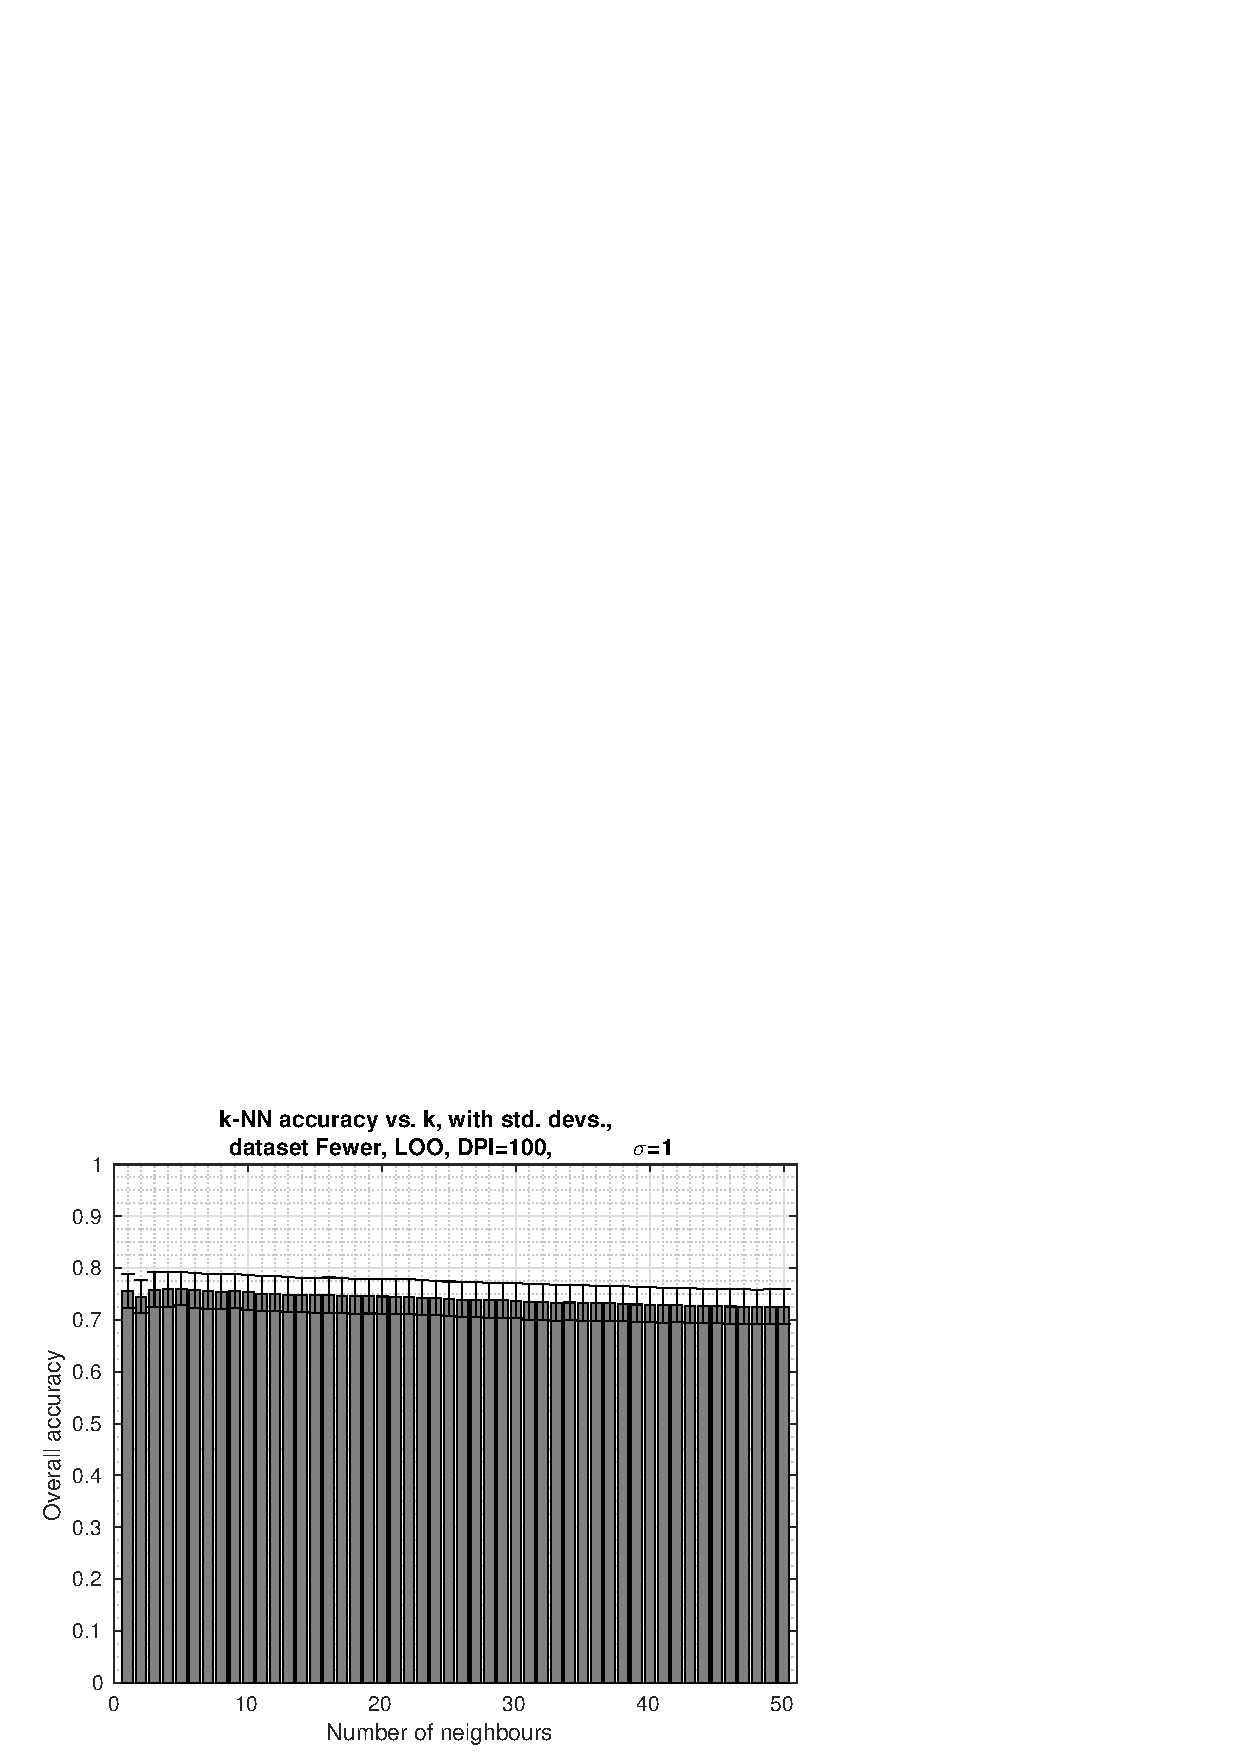
\includegraphics[width=\figscale]{img/pca-knn-acc-vs-k-dpi100-sigma1}
\caption[k-NN classification accuracy vs. k on $D_{FEWER}$, \textbf{LOO}.]
{
k-NN classification accuracy vs. k on $D_{FEWER}$, \textbf{LOO}, DPI=100, $\sigma=1$.
}
\label{fig:pca-knn-acc-vs-k}
\end{figure}

Figure \ref{fig:pca-svm-acc-vs-C} shows SVM classification accuracy vs.
cost of constraints violation C on the \(D_{FEWER}\) dataset.
It is observed that the accuracy does not vary significantly with C.
However, the maximal mean overall accuracy was found at C=0.5.
\begin{figure}[ht]
\centering
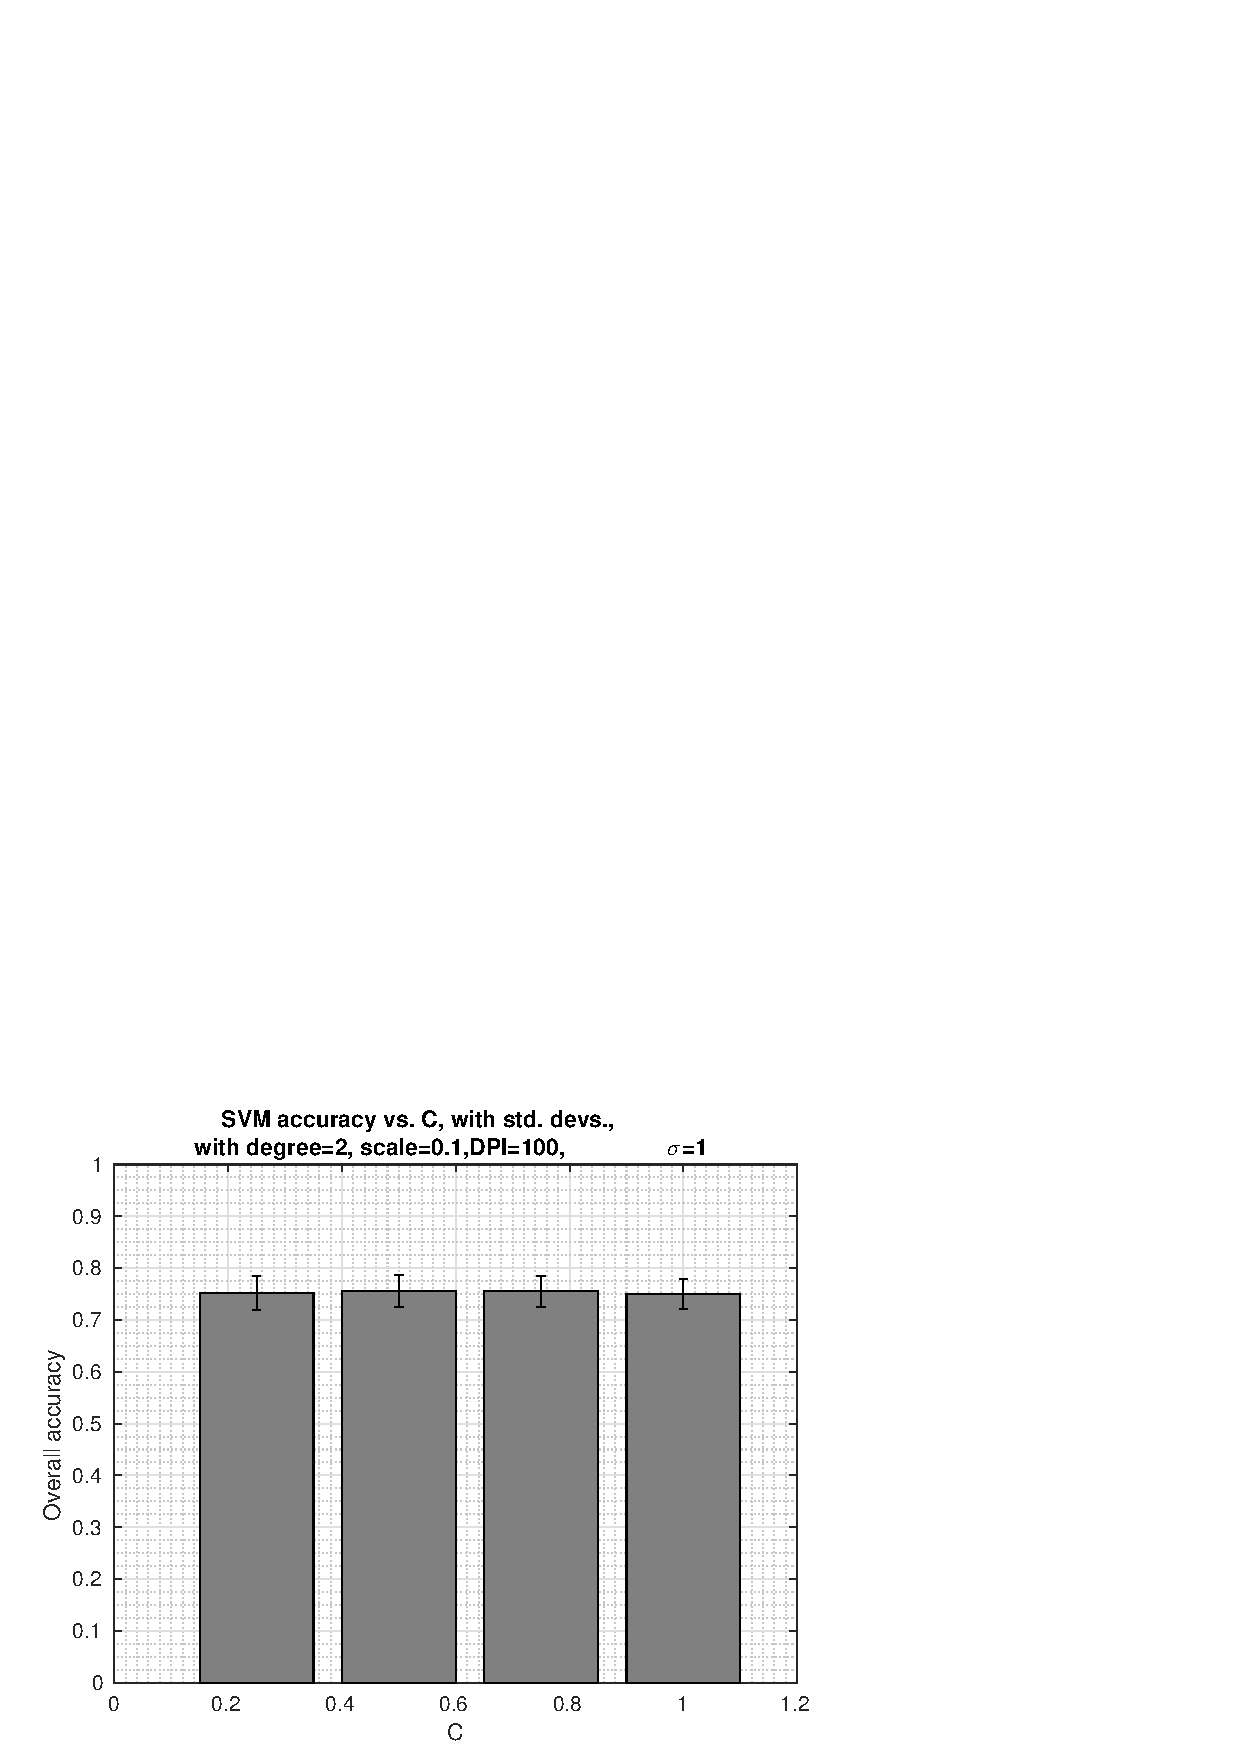
\includegraphics[width=\figscale]{img/pca-svm-acc-vs-C-dpi100-sigma1}
\caption[SVM classification accuracy vs. C on $D_{FEWER}$, \textbf{LOO}.]{
SVM classification accuracy vs. C on $D_{FEWER}$, \textbf{LOO}, DPI=100, $\sigma=1$.
The SVM kernel is polynomial with degree 2 and scale 0.1.
}
\label{fig:pca-svm-acc-vs-C}
\end{figure}

\clearpage
\subsection{Quality of individual datasets for classification}
Figure \ref{fig:singlePersonIndividual} shows k-NN and SVM
classification accuracy when applied to each persons dataset separately.
It is observed that the k-NN classification accuracy is lower than the SVM
classification accuracy on most of the datasets.
It is also observed that the lowest accuracy is found with data from \(G2M1\).
\begin{figure}[ht]
\centering
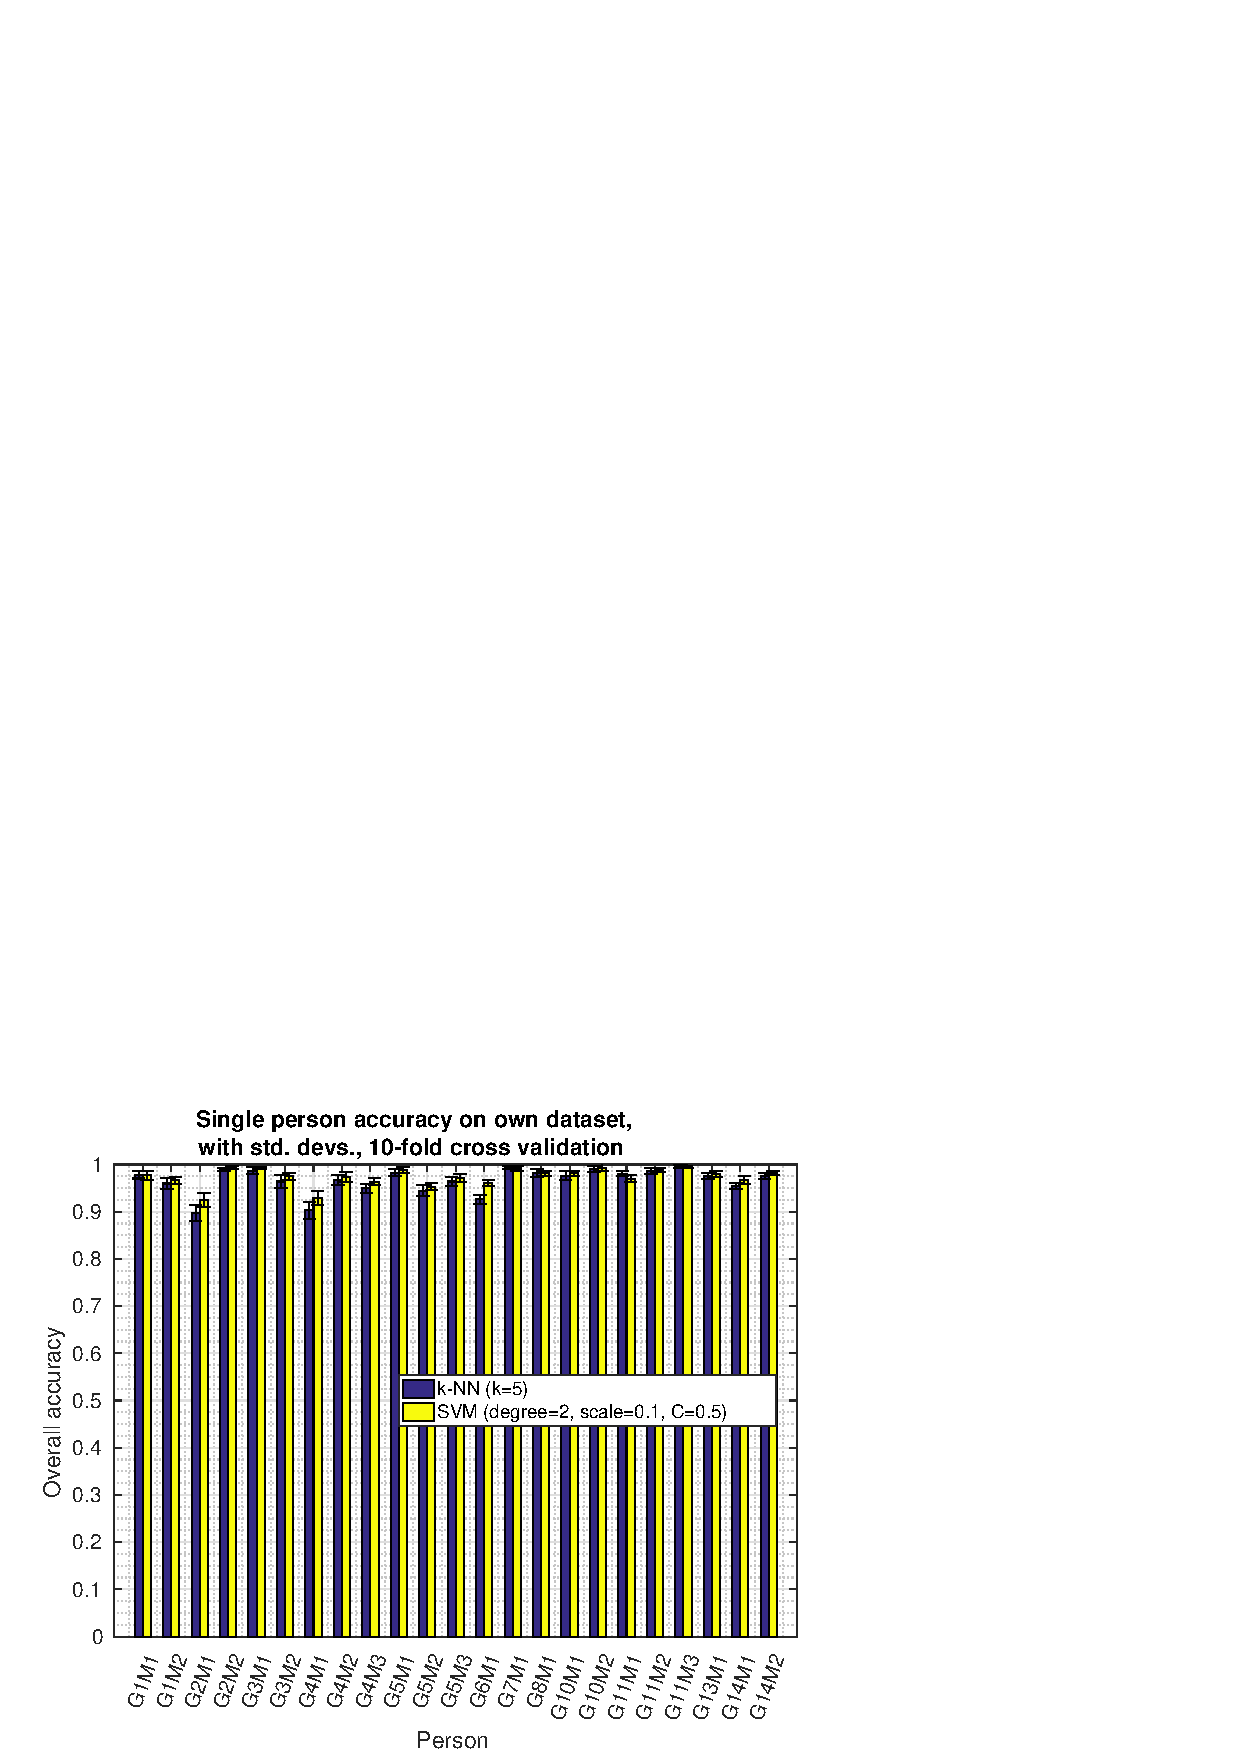
\includegraphics[width=\textwidth]{img/singlePersonIndividual-dpi100-sigma1}
\caption[Classification accuracy on individual datasets.]{
k-NN and SVM classification accuracy on each persons dataset, based on 10-fold cross validation.
}
\label{fig:singlePersonIndividual}
\end{figure}

\clearpage
\subsection{Comparison of classification algorithms}
k-NN and SVM classification accuracies are shown for three different
classification problems in figure \ref{fig:knn-vs-svm-full},
and a zoomed view is seen in figure \ref{fig:knn-vs-svm-zoomed}.
\begin{figure}[ht]
\centering
\begin{subfigure}{0.95\textwidth}
\centering
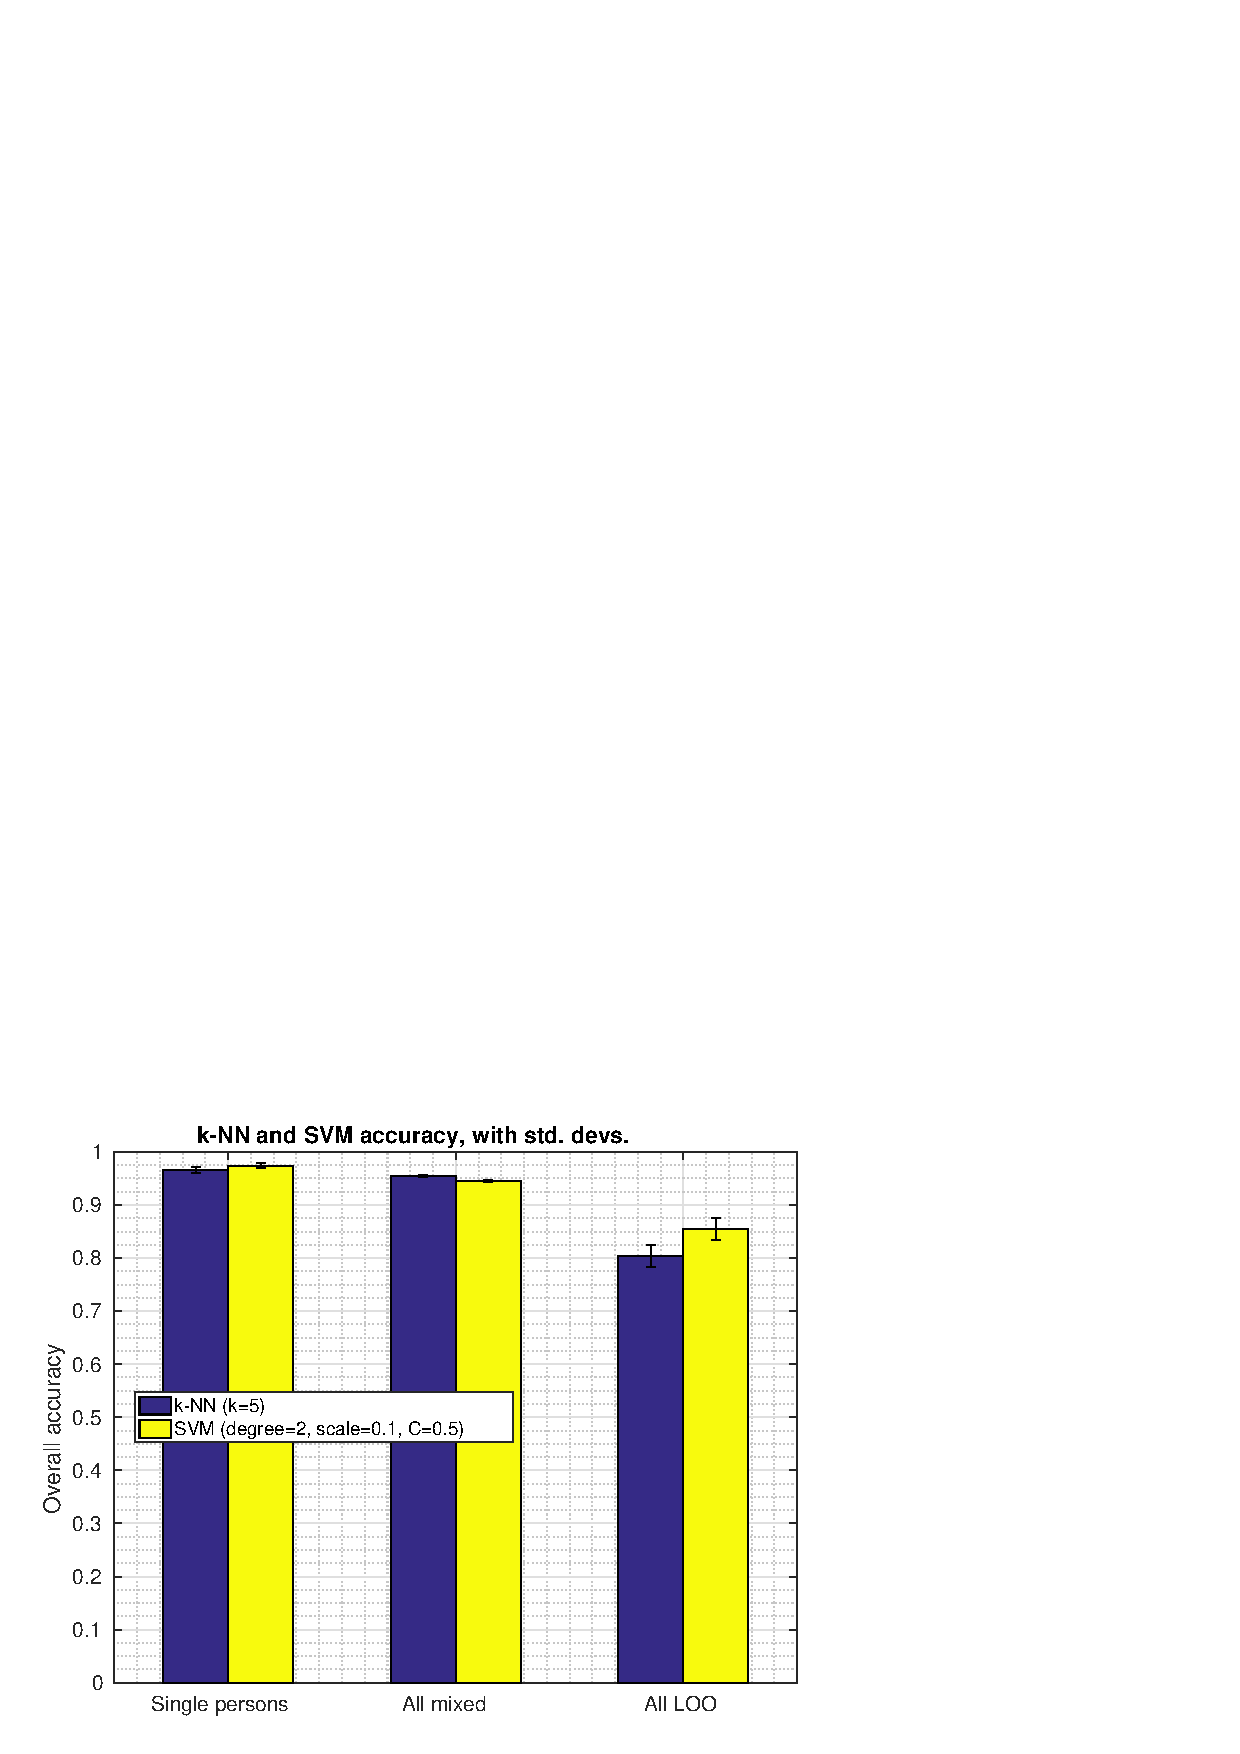
\includegraphics[width=\figscale]{img/knn-vs-svm-full-dpi100-sigma1}
\caption[k-NN and SVM classification accuracies, full view.]
{Full view.}
\label{fig:knn-vs-svm-full}
\end{subfigure}
\\
\vspace{0.5cm}
\begin{subfigure}{0.95\textwidth}
\centering
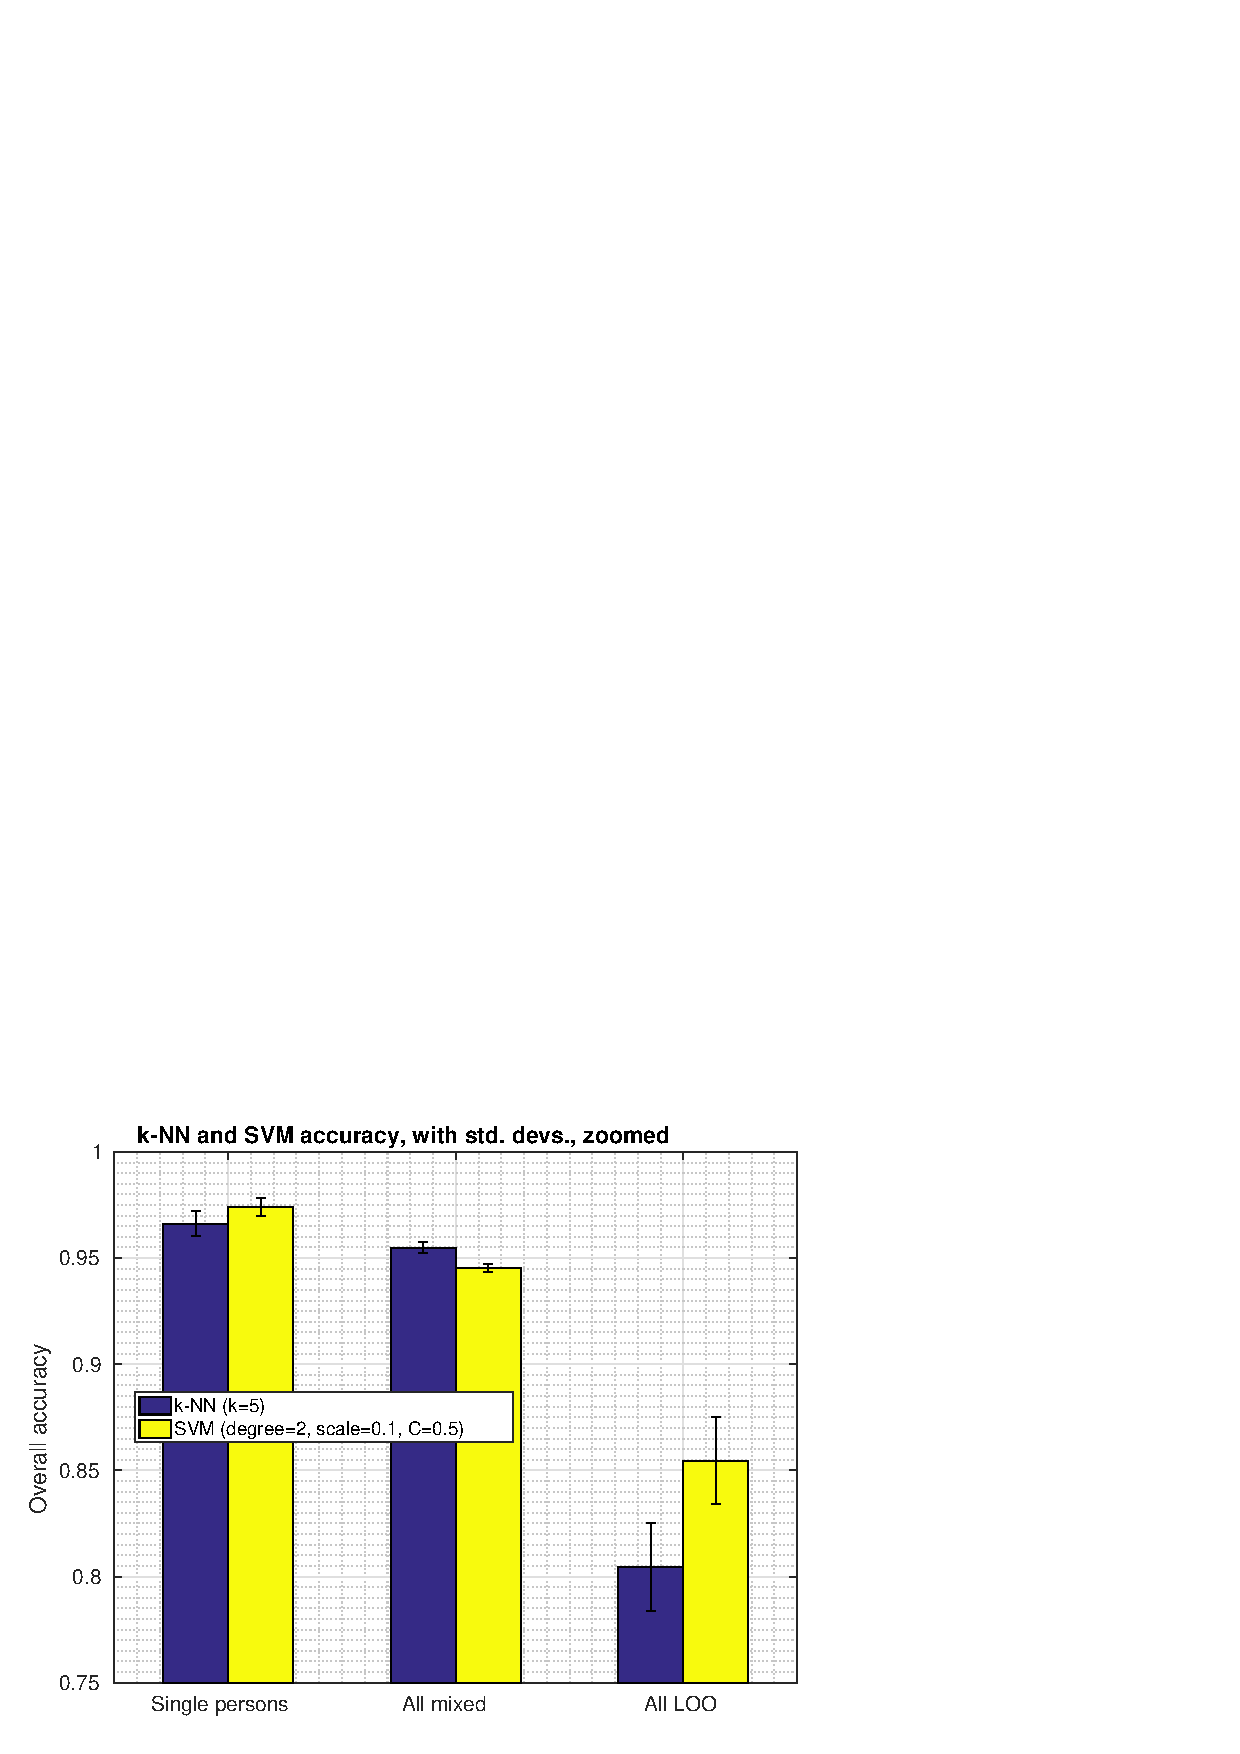
\includegraphics[width=\figscale]{img/knn-vs-svm-zoomed-dpi100-sigma1}
\caption[k-NN and SVM classification accuracies, zoomed view.]
{
Zoomed view.
}
\label{fig:knn-vs-svm-zoomed}
\end{subfigure}
\caption[k-NN and SVM classification accuracies]{
"Single persons" is the mean accuracy of the overall accuracy of 10-fold cross validation run for each individual.
"All mixed" is the mean accuracy based on $D_{ALL}$, \textbf{MIX}.
"All LOO" is the mean accuracy based on $D_{ALL}$, \textbf{LOO}.
The k-NN classifier was trained with k=5. The SVM classifier was trained with degree=2, scale=0.1 and C=0.5.
}
\end{figure}

For the "Single persons" problem, the SVM classifier has the highest mean accuracy.
For the "All mixed" problem, the k-NN classifier has the highest mean accuracy.
For the "All LOO" problem, the SVM classifier has the highest mean accuracy.

The highest observed accuracy for All LOO is 0.854 with a standard
deviation of 0.0205, for the SVM classifier.

The significance of these three results was tested by subtracting the classification
accuracies of the two algorithms from each other,
and applying a Z-test with a null hypothesis of zero mean.
With a level of significance \(\alpha=0.05\),
only the difference in the "All mixed" problem is significant.
The p-values of the three Z-tests are listed in table \ref{tb:ztest}.
\begin{table}[ht]
\centering
\caption[Z-test results]
{
Z-test results for the null hypotheses that k-NN accuracy has
the same mean as the SVM accuracy, \(H_0:\mu\left(\text{k-NN}\right)-\mu\left(\text{SVM}\right)=0\), for three different classification problems.
}
\begin{tabular}{|r||c|c|c|}
\hline
 & Single persons & All mixed & All LOO
 \\
 \hline
p-value & 0.28 & 0.0025 & 0.087
\\
CI (difference in accuracy)& \(\left[-0.022;0.0064\right]\)
& \(\left[0.0034;0.016\right]\)
& \(\left[-0.11;0.0072\right]\)
\\
\(H_0\) rejected & No & Yes & No
\\
\hline
\end{tabular}
\label{tb:ztest}
\end{table}

Figure \ref{fig:prediction-times} shows the prediction times per digit
of the k-NN and SVM classifiers, when trained with \(D_{ALL}\).
These prediction times were obtained by repeating the prediction
of all \(G2M2\) digits 30 times, taking the average and dividing by the number
of digits (4000).
It is observed from figure \ref{fig:prediction-times} that
the SVM classifier is more than twice as fast as the k-NN classifier,
when each is trained with \(D_{ALL}\).
\begin{figure}[ht]
\centering
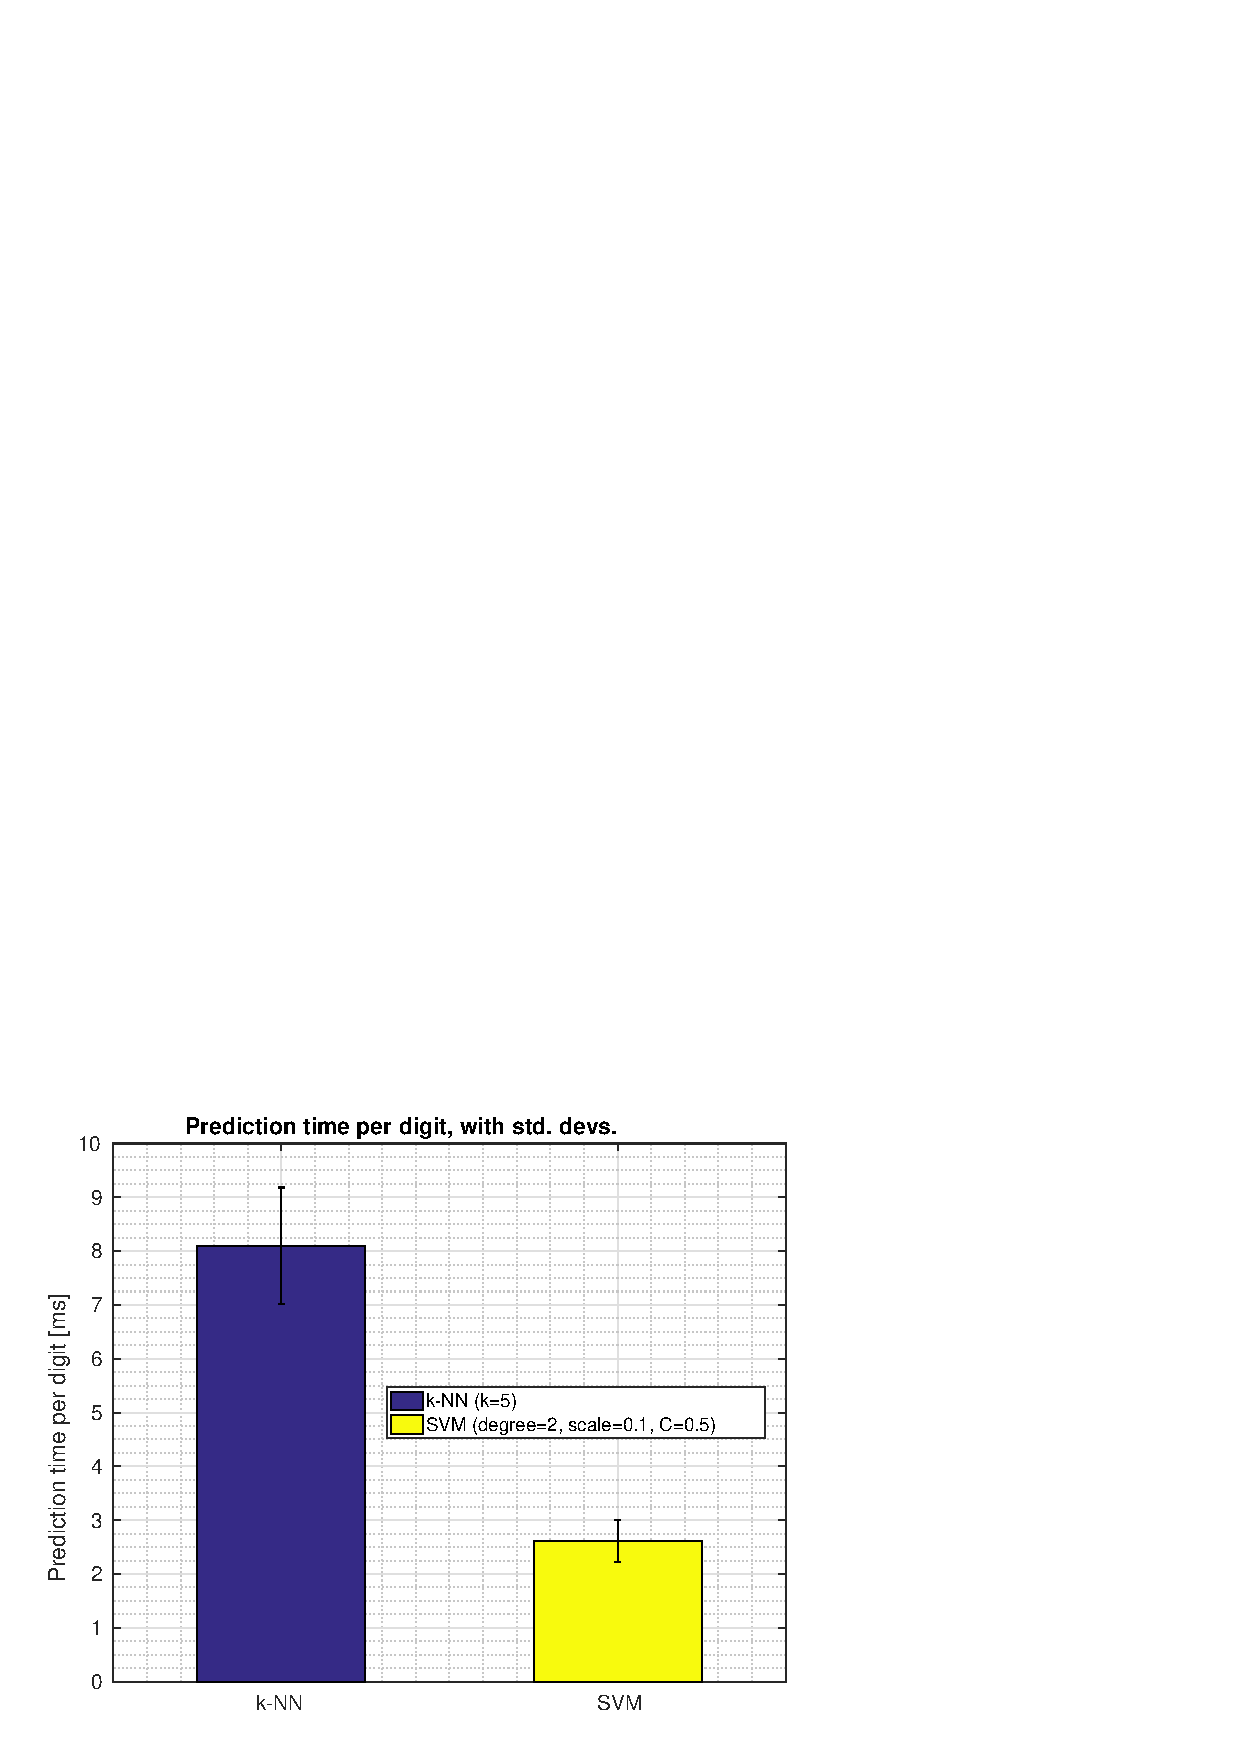
\includegraphics[width=\figscale]{img/prediction-times}
\caption[Prediction times per digit]
{
Prediction times per digit. Each classifier was trained with \(D_{ALL}\)
and applied to all \(G2M2\) digits 30 times.
The shown results are the average prediction times per digit.
}
\label{fig:prediction-times}
\end{figure}
%4000 digits:
%"knn_time_mean","knn_time_sdev","svm_time_mean","svm_time_sdev"
%32.4009333333333,4.32796005888043,10.4381333333333,1.58063548401692